\section{Vorgehen in Regelungstechnik}
Zur Ermöglichung einer strukturierten Vorgehensweise bedarf es einer Orientierung. Dieser Arbeit liegt die in der Vorlesung behandelte Vorgehensweise in der Regelungstechnik zugrunde, welche nachfolgend erläutert wird.

\begin{enumerate}
    \item Detaillierungsgrad für das System festlegen
    \item Physikalisches Modell einschließlich der Störsignale erstellen
    \item Eingangs-, Ausgangs-, Zustands- und Störgrößen des Systems festlegen
    \label{Punkt3}
    \item Physikalische Einheiten festlegen und ggf. Normierung in Prozent
    \label{Punkt4}
    \item Analyse des Modells
    \label{Punkt5}
    \begin{enumerate}
        \item Ruhelagen, Anfangswerte, evtl. Linearisierung nichtlinearer Systeme
        \item Systemeigenschaften ermitteln
    \end{enumerate}
    \item Entwurf
    \label{Punkt6}
    \begin{enumerate}
        \item Ziele, Arbeitspunkte und Trajektorien festlegen
        \item Entwurf: Struktur, Bereich, Verfahren und Kriterien
    \end{enumerate}
    \item Simulation und Rückinterpretation
    \label{Punkt7}
\end{enumerate}

In dieser Vorlesung wird die Regelungstechnik außen vor gelassen, weswegen im Folgenden eine leicht abgewandelte Struktur angewendet wird. Bezüglich des Detaillierungsgrads sind alle in der Vorlesung behandelten Darstellungsformen darzulegen. Weiterführend werden die Punkte \hyperref[Punkt3]{3} und \hyperref[Punkt4]{4} des Vorgehens aus der Regelungstechnik zusammengefasst und tabellarisch dargestellt. Schwerpunktmäßig wird in dieser Arbeit Punkt \hyperref[Punkt5]{5} behandelt, in dem alle Darstellungsformen aus der Vorlesung dargelegt werden. Punkt \hyperref[Punkt6]{6} und \hyperref[Punkt7]{7} werden in dieser Arbeit nicht betrachtet.

\section{Unser System}
Wir betrachten einen Wassertank, der oben an einen Zufluss mit sehr hohem Druck angeschlossen ist. Am unteren Ende des Wassertanks befindet sich ein deutlich kleinerer Abfluss, an den eine lange Wasserleitung angeschlossen ist. Erst am Ende der Wasserleitung befindet sich das Messgerät, welches den Volumenstrom misst. \\
Eine beispielhafte Skizze sieht folgendermaßen aus:
\begin{figure}[H]
    \label{fig:tank}
    \centering
    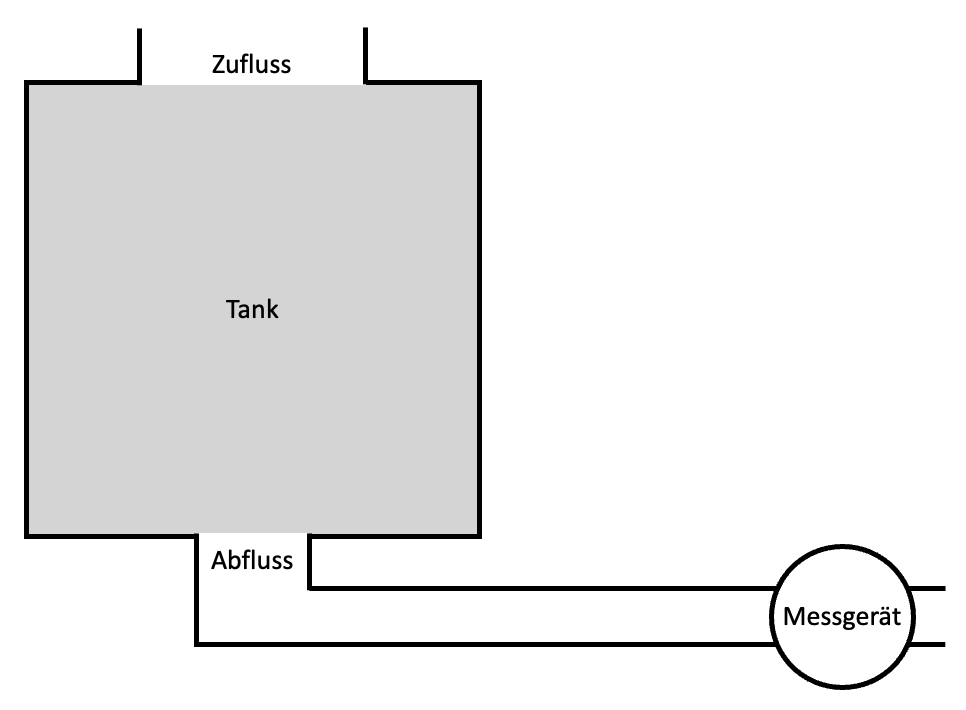
\includegraphics[width=0.6\textwidth]{Bilder/Tank.png}
    \caption{Skizze des Systems}
 \end{figure}
Der Ablauf stellt sich wie folgt dar: Über den Zufluss fließt Wasser in den Tank. Da der Abfluss aber deutlich kleiner ist, fließt erstmal deutlich weniger Wasser heraus. Erst wenn der Tank voller wird, erhöht sich der Druck und es kommt zu einem immer größeren Volumenstrom. Schließlich ist der Tank so voll (Wasser und komprimierte Luft), dass der Druck des Zuflusses dafür sorgt, dass der Volumenstrom am Abfluss gleich dem am Zufluss ist. Da das Messgerät aber weit entfernt vom Tank liegt, misst dieses den ganzen Vorgang erst mit einer gewissen Verzögerung.

Je nachdem wie groß der Tank ist, verändert sich die Konstante $T_1$: Je kleiner der Tank, desto größer ist $T_1$. Aber auch das Verhältnis von Zuflussgröße zu Abflussgrößte beinflusst die Konstante $T_1$. Gleichzeitig bestimmt der Abstand zwischen dem Tank und dem Messgerät die Zeitkonstante $T_t$: Je größer der Abstand, destor größer ist $T_t$.

\subsection{Größen}
Im Folgenden werden Eingangs-, Zustands- und Ausgangsgrößen des Systems definiert.
\renewcommand{\arraystretch}{1.5}
\begin{center}
    \begin{tabular}{ c|c|l } 
    Systemtheorie  & Größe im System & Einheit \\
    \hline
    $u(t)$ & Volumenstrom am Zufluss & $\frac{l}{min}$ \\ 
    $x(t)$ & Volumenstrom am Abfluss &  $\frac{l}{min}$\\ 
    $y(t)$ & Volumenstrom am Messgerät & $\frac{l}{min}$ \\ 
    \end{tabular}
\end{center}
%Die Eingangsgröße $u(t)$ ist in unserem Beispiel der Volumenstrom am Zufluss, angegeben z.\,B. in $\frac{l}{min}$. Der Zustand $x(t)$ ist der Volumenstrom am Abfluss und der Ausgang $y(t)$ ist der gemessene Volumenstrom am Messgerät.


\subsection{Bezeichnung}
Das System hat den Nennergrad 1, eine Totzeit $T_t$ und ein proportionales Übertragungsverhalten. Daraus ergibt sich die Bezeichnung $PT_{1}T_{t}$.

\subsection{Übertragungsfunktion}

Formel \ref{eq:G(s)_1} zeigt die Übertragungsfunktion die in diesem Skript analysiert wird. Dabei gehen wir bei unserem System gehen davon aus, dass $T_1$ gleich 1 und $T_t$ gleich 2 ist. Formel \ref{eq:G(s)_3} zeigt eine etwas andere Darstellung der Formel, sodass die Eigenschaften des Systems leichter abzulesen sind.

\begin{eqnarray}
    \label{eq:G(s)_1}
    \mathcal{G}(s) &=& \frac{Y(s)}{U(s)} \\
    \label{eq:G(s)_2}
    &=& \frac{1 \cdot e^{-2s}}{1+s} \\
    \label{eq:G(s)_3}
    &=& \frac{1}{1 + s} \cdot e^{-2s}
\end{eqnarray}

\subsection{Eingabe in Matlab}
Für die Eingabe der Übertragungsfunktion in Matlab gibt es zwei Möglichkeiten. \\
In Computer-Algebra führt man \texttt{s} und \texttt{G(s)} als symbolischen Variablen ein und kann anschließend die Übertragungsfunktion \texttt{G(s)} definieren:

\begin{verbatim}
    syms s, G(s)
    G(s) =  1 / (1 + s) * exp(-2 * s)
\end{verbatim}

Man erhält dasselbe Ergebnis wie bei der obigen manuellen Definition von $s$ und $\mathcal{G}(s)$, wenn man den Transfer-Function-Befehl \texttt{tf()} in Matlab verwendet:

\begin{verbatim}
    sys = tf([1], [1, 1], "IODelay", 2)
\end{verbatim}

Hierbei werden in den beiden Vektoren die Koeffizienten vor $s^0$, $s^1$, $s^2$, \ldots im Zähler und im Nenner angegeben. Bei komplizierteren Gleichungen hilft dabei der Befehl \texttt{expand(G(s))}, der einem die benötigten Koeffizienten liefert, was hier jedoch nicht nötig war. \\
Darauf folgt der Befehl \texttt{\textquotedbl IODelay\textquotedbl}, mit dem die Totzeit $t = 2$ angegeben wird.

\section{Darstellungsformen des Systems}
Im Folgenden werden die Darstellungen unseres Systems näher beleuchtet. Generell gilt: Mit jeder weiteren Darstellung verliert man bestimmte Informationen über das System, sodass die erste Darstellung die informationsreichste ist.

\subsection{Explizite Darstellung des Übertragungsoperators}

Mit den Anfangswerten lässt sich $x(t)$ und $y(t)$ explizit berechnen:

\begin{align*}
    x(t) & = e^{At} \cdot x(0) + \int_{0}^{t} e^{A(t-\tau)}Bu(\tau) \,d\tau \nonumber \\
    y(t) & = Ce^{At} \cdot x(0) + C \int_{0}^{t} e^{A(t-\tau)}Bu(\tau) \,d\tau + Du(t)
\end{align*}

Hier ist bei der Eingabe in Matlab wichtig zu beachten, dass für $e^{(\ldots)}$ nicht \texttt{exp}, sondern \texttt{expm}, verwendet wird, da man hier die Matrizenmultiplikation benötigt.

Für unsere System ergibt sich durch Einsetzen der jeweiligen Werte und der Heaviside-Funktion als Eingang:

\noindent
\begin{minipage}{.5\linewidth}   
    \begin{align*}
        x(t) & = \int_{0}^{t} \begin{bmatrix}e^{-t + \tau}\end{bmatrix} \,d\tau \\
        x(t) & = \int_{0}^{t} \begin{bmatrix}e^{-t} \cdot e^{\tau}\end{bmatrix} \,d\tau \\
        x(t) & = e^{-t} \cdot e^{t} - e^{-t} \cdot e^{0} \\
        x(t) & = 1 - e^{-t}
    \end{align*}
\end{minipage}
\begin{minipage}{.5\linewidth}   
    \begin{align*}
        y(t) & = \int_{0}^{t} \begin{bmatrix}e^{-t + \tau}\end{bmatrix} \,d\tau \\
        y(t) & = \int_{0}^{t} \begin{bmatrix}e^{-t} \cdot e^{\tau}\end{bmatrix} \,d\tau \\
        y(t) & = e^{-t} \cdot e^{t} - e^{-t} \cdot e^{0} \\
        y(t) & = 1 - e^{-t}
    \end{align*}
\end{minipage}

\subsection{Implizite Darstellung}
\subsubsection{Zustandsraumdarstellung}
Die allgemeine Form der Zustandsraumdarstellung lautet:
\begin{align*}
    \dot x & = Ax + Bu \nonumber \\
    y & = Cx + Du
\end{align*}

Mit dem Matlab-Befehl \texttt{ss(sys)} (ss für State Space) berechnet Matlab die Zustandsmatrizen für unser System. Somit ergibt sich die folgende Zustandsraumdarstellung:
\begin{align*}
    \dot x & = \begin{bmatrix}
        -1
    \end{bmatrix}x + \begin{bmatrix}
        1
    \end{bmatrix}u \\
    y & = \begin{bmatrix}
        1
    \end{bmatrix}x + \begin{bmatrix}
        0
    \end{bmatrix}u
\end{align*}

Sind die Zustandsmatrizen eines Systems bekannt, kommt man mit der folgenden Formel zur Übertragungsfunktion $\mathcal{G}(s)$, wobei $I$ die Einheitsmatrix darstellt.
\[
    \mathcal{G}(s) = C(s \cdot I - A)^{-1} \cdot B + D
\]

Sofern die Zustandsmatrizen gegeben sind, kann man das System alternativ mit der dazugehörigen Zustandsraumdarstellung übergeben, indem \texttt{sys = ss(A, B, C, D)} in Matlab eingegeben wird. Der Befehl \texttt{tf(sys)} liefert dann die Übertragungsfunktion.

In unserem System erhält man damit aber nicht die eigentliche Übertragungsfunktion, da die Totzeit $T_t$ verloren geht.

Für die Funktionalbeziehung eines Totzeitglieds im Zeitbereich gilt: $y(t) = u(t-T_t)$. \\
Somit ergibt sich für die Zustandsraumdarstellung eines zeitverzögerten Systems:
\begin{align*}
    \dot x(t) & = Ax(t) + Bu(t - T_t) \nonumber \\
    y(t) & = Cx(t) + Du(t - T_t)
\end{align*}
In unserem System mit $T_t = 2$ bedeutet das:
\begin{align*}
    \dot x(t) & = \begin{bmatrix}
        -1
    \end{bmatrix}x(t) + \begin{bmatrix}
        1
    \end{bmatrix}u(t - 2) \nonumber \\
    y(t) & = \begin{bmatrix}
        1
    \end{bmatrix}x(t) + \begin{bmatrix}
        0
    \end{bmatrix}u(t - 2)
\end{align*}

Anhand der Matrix $D$, die in unserem System eine Nullmatrix ist, lässt sich ablesen, dass es sich hier um ein nicht sprungfähiges System handelt.

Ohne Matlab kann die Zustandsraumdarstellung in einfachen Fällen mithilfe des Substitutionstricks aus der Übertragungsfunktion errechnet werden. Für Systeme, bei denen auch $\dot u, \ddot u, \ldots$ in der Differentialgleichung vorkommt, ist das Ganze ein bisschen komplizierter, wird aber in \href{https://de.wikipedia.org/wiki/Zustandsraumdarstellung#Regelungsnormalform}{Wikipedia} beschrieben und kann entsprechend angewendet werden. Bei sprungfähigen Systemen sieht das noch etwas anders aus und es muss erst eine Polynomdivision gemacht werden, um $D$ zu erhalten. Im Mehrgrößenfall ist es noch komplizierter.

\subsubsection*{Anfangswerte}

Für die Simulation sind Anfangswerte notwendig, da der Start der Funktion definiert sein muss. Hierbei werden die linkseitigen Grenzwerte verwendet, da sonst eventuelle Sprünge miteinbezogen würden. Es gilt:
\begin{align*}
    y(0^-) & = Cx(0^-) + Du(0^-) \\
    \dot y(0^-) & = CAx(0^-) + CBu(0^-) + D \dot u (0^-)
\end{align*}

Die Summanden, in denen $\dot u, \ddot u, \ldots$ vorkommt, können vernachlässigt werden. Schließlich sind die linksseiten Anfangswerte aufgrund der Heavyside-Funktion gleich 0.

Darüber hinaus gibt es einen Zusammenhang mit der Ein-/Ausgangs-Differentialgleichung: Die Anfangswerte des Zustandsraumes $x$ müssen mit denen der Ein-/Ausgangs-Differential-gleichung $y$ korrespondieren. Zur Berechnung werden folgende Formeln verwendet:

\begin{align*}
    \left(\begin{array}{c} y \\ \dot y \\ \ddot y \end{array}\right) &= \left(\begin{array}{l} c^T \\ c^T A \\ c^T A^2 \end{array}\right) \left(\begin{array}{c} x_1 \\ x_2 \\ x_3 \end{array}\right) \\
    \left(\begin{array}{c} x_1 \\ x_2 \\ x_3 \end{array}\right) &= \left(\begin{array}{l} c^T \\ c^T A \\ c^T A^2 \end{array}\right)^{-1} \left(\begin{array}{c} y \\ \dot y \\ \ddot y \end{array}\right)
\end{align*}

Weiterhin gehen wir bei unserem System davon aus, dass der Tank zu Beginn leer ist, somit kein Abfluss vorliegt. Daraus ergibt sich $x(0^-) = 0$ und mit voriger Formel gilt:
\begin{align*}
    \left(\begin{array}{c} y \\ \dot y \end{array}\right) &= \left(\begin{array}{c}0\\0\end{array}\right) \\
    \left(\begin{array}{c} x_1 \\ x_2 \end{array}\right) &= \left(\begin{array}{c}0\\0\end{array}\right)
\end{align*}


\subsubsection{Integralgleichung}
Im Gegensatz zur Differentialgleichung ergibt die Integralgleichung \enquote{mild solutions}, welche Sprünge abbilden können. Sie lässt durch Integration der Differentialgleichung mit $\int_{0}^{t}$. \\ 
Für die Integralgleichung gilt:

\noindent
\begin{minipage}{.5\linewidth}   
    \begin{align*}
        x(t) & = x(0) + \int_{0}^{t} Ax(\tau) + Bu(\tau)\,d\tau
    \end{align*}
\end{minipage}
\begin{minipage}{.5\linewidth}   
    \begin{align*}
        y(t) & = y(0) + \int_{0}^{t} Cx(\tau) + Du(\tau)\,d\tau
    \end{align*}
\end{minipage}

Für unser System ergibt sich somit:

\noindent
\begin{minipage}{.5\linewidth}   
    \begin{align*}
        x(t) & = \int_{0}^{t} \begin{bmatrix}
            -1
        \end{bmatrix}x(\tau) + \begin{bmatrix}
            1
        \end{bmatrix}u(\tau)\,d\tau
    \end{align*}
\end{minipage}
\begin{minipage}{.5\linewidth}   
    \begin{align*}
        x(t) & = \int_{0}^{t} \begin{bmatrix}
            -1
        \end{bmatrix}x(\tau) + \begin{bmatrix}
            1
        \end{bmatrix}u(\tau)\,d\tau
    \end{align*}
\end{minipage}

\subsubsection{Differentialgleichung}
Aus unserem physikalischen Modell lässt sich folgende Differentialgleichung ableiten:
\begin{align*}
    \dot x & = u - x \enspace \enspace \enspace \enspace \enspace \enspace \enspace \text { mit } x(0) = 0\\
    y(t) & = x(t - 2) \\
\end{align*}

\subsection{Ein-/Ausgangs Differentialgleichung}
Für unser System ergibt sich unter Vernachlässigung des Totzeitglieds:
\begin{align*}
G_{PT_1}(s) =\frac{Y(s)}{U(s)} &= \frac{1}{1 + s} \\
Y(s)(1+s) &= (1) \cdot U(s) \\
Y(s) + Y(s) \cdot s &= 1\cdot U(s) \\
\dot y(t) + y(t) &= u(t) 
\end{align*}

In dieser Differentialgleichung taucht die Totzeit $T_t$ nicht auf, da das Totzeitglied nicht mit einer gewöhnlichen Differentialgleichung beschrieben werden kann. Für die Funktionalbeziehung eines Totzeitglieds im Zeitbereich gilt: $y(t) = u(t-T_t)$. \\
Für unser System mit der Totzeit $T_t = 2$ folgt somit:
\begin{align*}
    \dot y(t) + y(t) &= u(t - 2) \enspace \enspace \enspace \enspace \enspace \enspace \enspace \text { mit } y(0) = 0
\end{align*}

\subsection{Übertragungsfunktion}
Die Übertragungsfunktion ergibt sich durch die Laplace-Transformation der Ein-/Ausagangs-Differentialgleichung, wird für unser System in Kapitel 2.3 definiert und lautet: 

\begin{align*}
    \mathcal{G}(s) &= \frac{1}{1 + s} \cdot e^{-2s} 
\end{align*}

\subsection{Systemantworten}
Im Folgenden werden die Antworten des Systems auf den Dirac-Impuls $\delta(t)$ und den Einheitssprung $\sigma (t)$ näher erläutert.
Die Sprungantwort $h(t)$ und die Impulsantwort $g(t)$ sind jeweils ineinander überführbar: Durch Differenzieren von $h(t)$ erhält man $g(t)$ und durch Integrieren von $g(t)$ erhält man $h(t)$.
\subsubsection{Gewichtsfunktion (Impulsantwort)}
Die Impulsantwort bezeichnet die abgetastete Antwort auf den technischen Dirac-Impuls.
Die Gewichtsfunktion $g(t)$ ist die Antwort eines Sytems auf einen Dirac-Impuls.

In Matlab lässt sich die Gewichtsfunktion sowohl graphisch als auch analytisch ausgeben.
\texttt{ilaplace()} liefert die inverse Laplace-Transformation der Übertragungsfunktion:
\begin{verbatim}
    syms g(t)
    g(t) = ilaplace(G(s))
\end{verbatim}

Matlab Ausgabe: \texttt{g(t) = heaviside(t - 2) * exp(2 - t)}\\
Mathematische Notation: 
\begin{align*}
    g(t) &=1(t-2)\cdot e^{(2-t)}
\end{align*} wobei $1(t)$ für die Heavyside-Funktion steht.

Einen Plot der Impulsantwort erhält man mit \texttt{impulse(sys)}.

\begin{figure}[H]
    \label{fig:impuls}
    \centering
    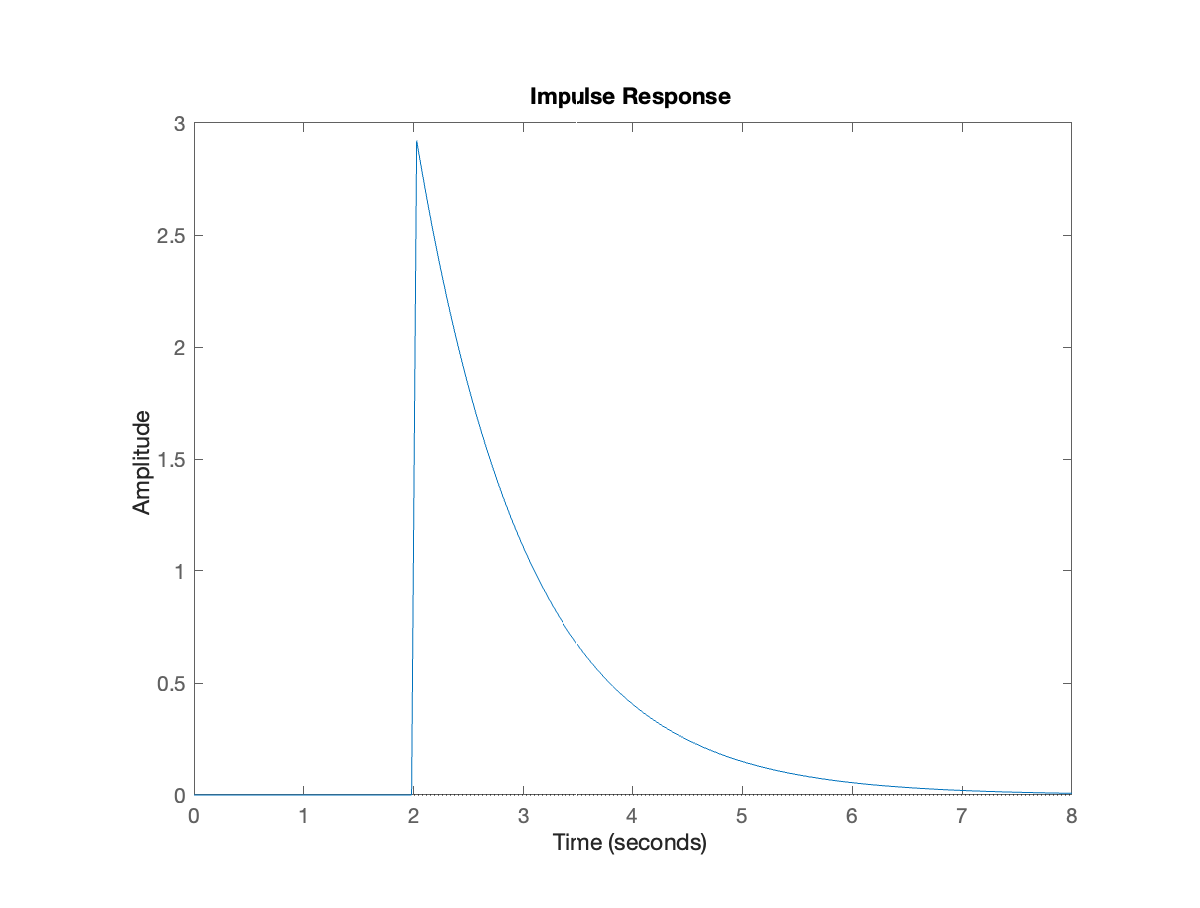
\includegraphics[width=0.8\textwidth]{Bilder/ImpulsAntwortPT1Tt.eps}
    \caption{Impulsantwort}
 \end{figure}

\subsubsection{Übergangsfunktion (Sprungantwort)}

Die Spungantwort bezeichnet die Antwort des Systems auf den technischen Einheitssprung.
Die Übergangsfunktion $h(t)$ ist somit die einheitenlose Antwort des Systems auf den Einheitssprung.
Ein Beipsiel ist die Heaviside-Funktion, die wie folgt definiert ist:

\[
1 (t) = \begin{cases} 
    0 & \text{für t < 0} \\ 
    \frac{1}{2} & \text{für t = 0} \\
    1 & \text{für t > 0} \end{cases}  
\]

In Matlab lässt sich das mit dem Befehl \texttt{step(sys)} simulieren, wodurch man die numerische Lösung erhält, wie in folgender Abbildung zu sehen.

\begin{figure}[H]
    \label{fig:sprung}
    \centering
    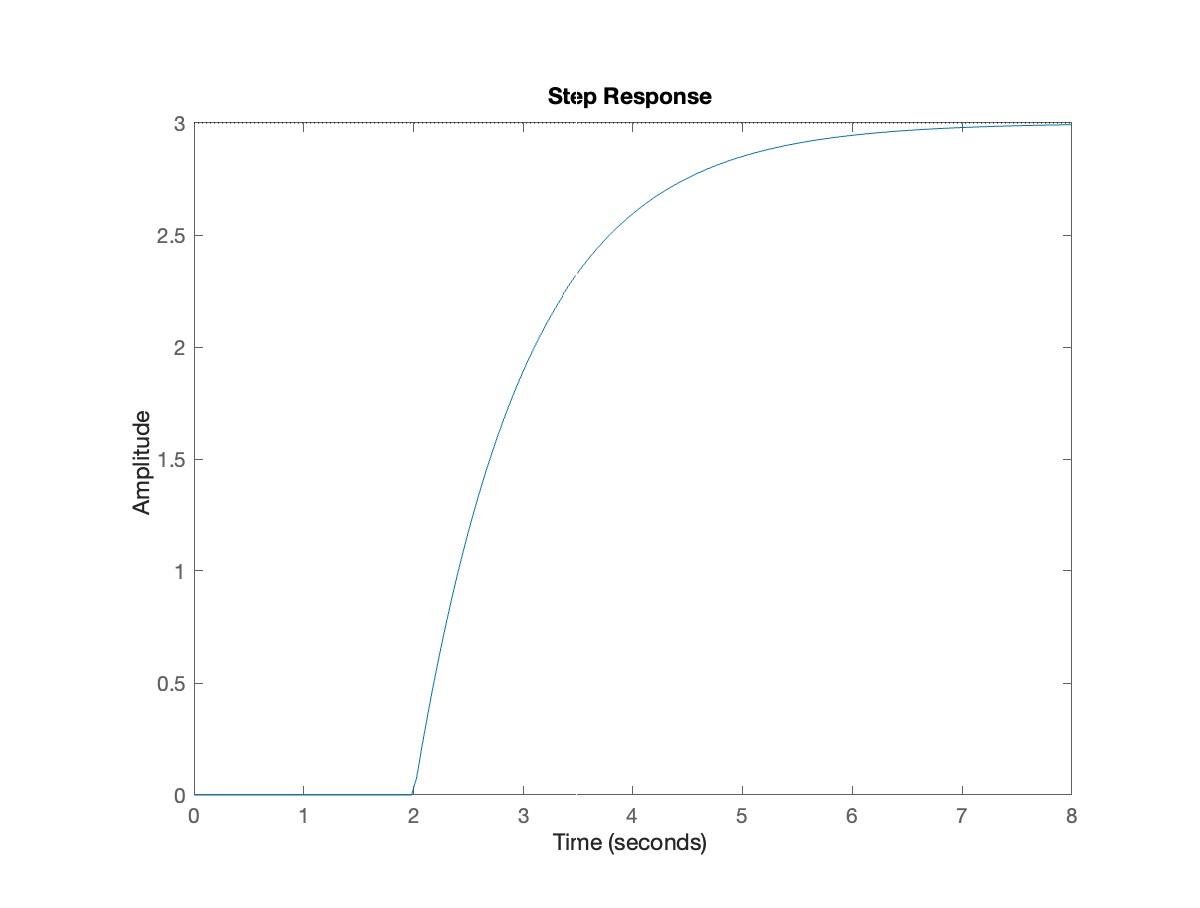
\includegraphics[width=0.8\textwidth]{Bilder/SprungantwortPT1Tt.eps}
    \caption{Sprungantwort}
 \end{figure}

Die Übergangsfunktionfunktion $h(t)$ lässt sich aber auch analytisch berechnen und man erhält die explizite Lösung.

\begin{verbatim}
    H(s) = G(s)/s
    syms h(t)
    h(t) = ilaplace(H(s))
\end{verbatim} 

Matlab Ausgabe: \texttt{h(t) = -heaviside(t - 2) * (exp(2 - t) - 1)}\\
Mathematische Notation: 
\begin{align*}
    h(t) &= -1(t-2)\cdot(e^{(2-t)}-1)
\end{align*}


\subsection{Frequenzgang}
Zum Frequenzgang $G(j \omega)$ gelangt man, indem man in $\mathcal{G}(s)$ die Variable $s$ durch $j \omega$ ersetzt.\\
Das $\omega$ steht für die Frequenz in $\frac{rad}{s}$ (Erinnerung: $\omega = 2\pi f$). Das $j$ steht für die imaginäre Einheit, da $i$ in der Systemtheorie für den Strom steht und somit durch $j$ ersetzt wird.

Das bedeutet, dass $G(j \omega)$ für jede Frequzenz $\omega$ eine komplexe Zahl $j$ mit Real- und Imaginärteil oder einen Betrag mit Phase darstellt.
Systemtheoretisch entspricht der Frequenzgang $G(j\omega)$ einem Schnitt der komplexen Funktion von $\mathcal{G}(s)$ entlang der imaginären Achse: $\mathcal{G}(s)|_{s = j * \omega}$

\subsubsection{Nyquist-Plot (Ortskurve)}
Im Nyquist-Plot wird der über $\omega$ parametrisierte Frequenzgang als Kurve in der komplexen Ebene mit Real- und Imaginärteil dargestellt.

Mit dem Matlab-Befehl \texttt{nyquist(sys)} wird ein Plot der Kurve des Frequenzgangs $G(\omega j)$ ausgegeben. 
Matlab zeigt die Kurve des Frequenzgangs $G(j\omega)$ immer für $\omega$ zwischen $- \infty$ und $+ \infty$ an:

\begin{figure}[H]
    \label{fig:nyquist}
    \centering
    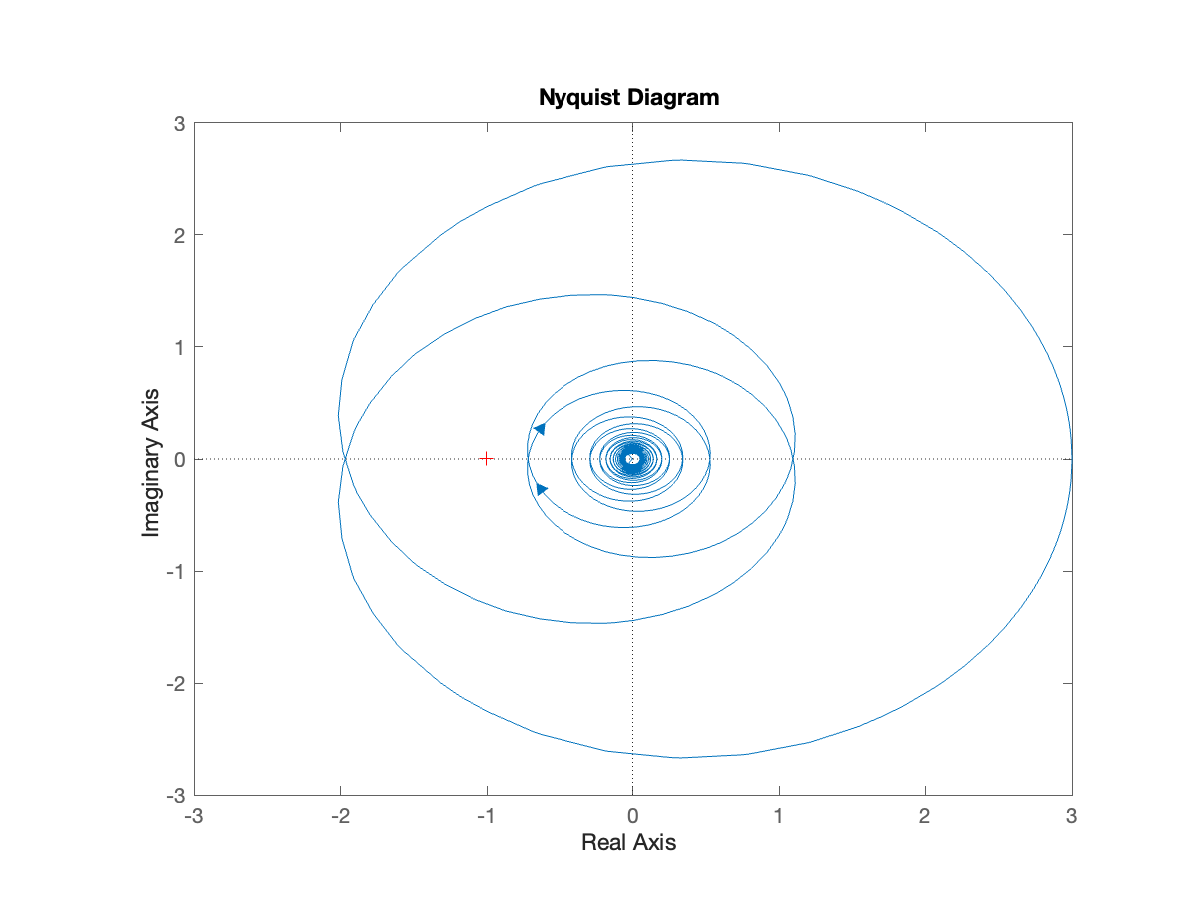
\includegraphics[width=0.8\textwidth]{Bilder/NyquistPT1Tt.eps}
    \caption{Nyquist-Plot}
 \end{figure}

 Dabei ist es möglich, mit dem Cursor entlang der Kurve zu fahren, um sich den Real- und Imaginärteil zu dem jeweiligen Punkt anzeigen zu lassen:
 \begin{figure}[H]
    \label{fig:nyquistCursor}
    \centering
    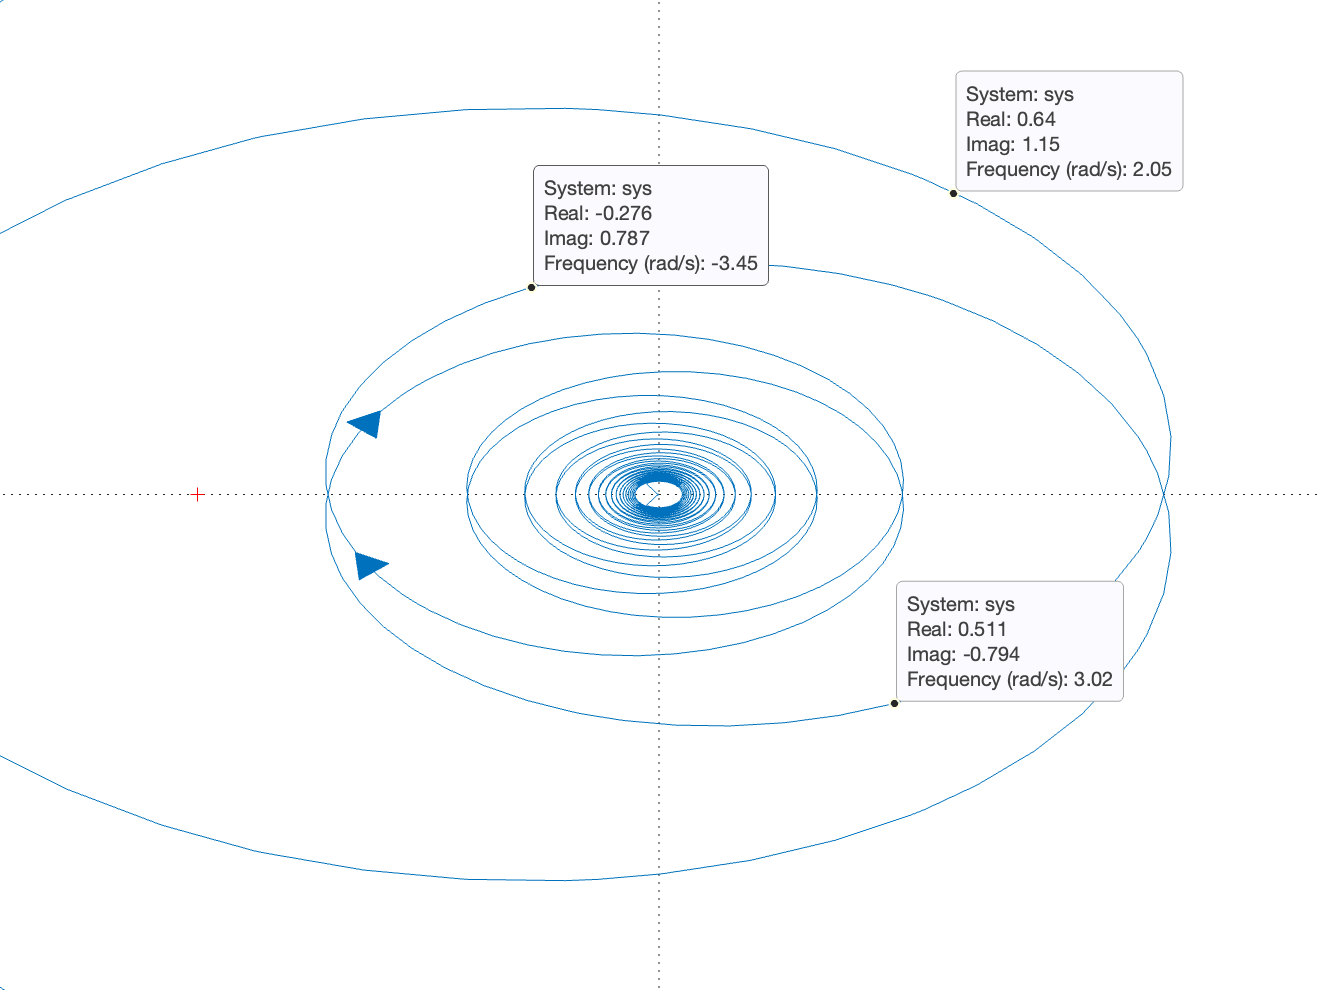
\includegraphics[width=0.6\textwidth]{Bilder/NyquistCursorPT1Tt.png}
    \caption{Screenshot: Informationen im Nyquist-Plot}
 \end{figure}

 
\subsubsection{Bode-Diagramm}
Im Bode-Diagramm sind der Betrag des Frequenzgangs über $\omega$ in Dezibel ($dB$) und die Phase des Frequenzgangs über $\omega$ in Grad ($^\circ$) dargestellt.\\
Streng genommen wird im oberen Diagramm der Abbildung 6 die Amplitudenverstärkung dargestellt, die ein Sinus-Signal an der Frequenz $\omega$ stationär erfährt (wenn die Eigenvorgänge abgeklungen sind und sich das System eingeschwungen hat), während im unteren Diagramm die Phasenverschiebung zu sehen ist.  

Der dazugehörige Matlab-Befehl ist \texttt{bode(sys)}, wobei dieser Befehl intern eine doppelt logarithmische Darstellung verwendet. Die Diagramm-Achse, auf der $\omega$ aufgetragen ist, ist dabei logarithmisch skaliert, damit die Kurven schön aussehen.

\begin{figure}[H]
    \label{fig:bodePlot}
    \label{fig:lassmich}
    \centering
    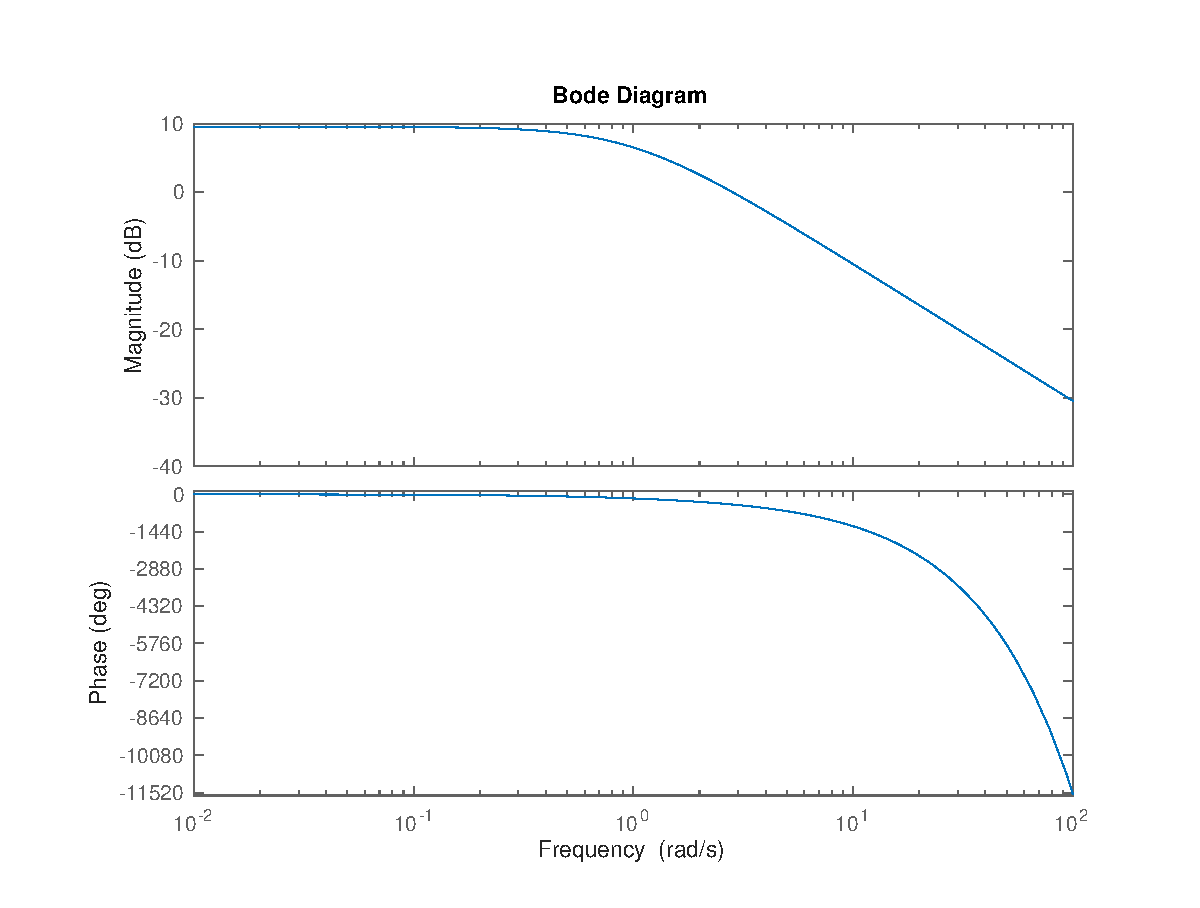
\includegraphics[width=0.8\textwidth]{Bilder/BodePT1Tt.eps}
    \caption{Bode-Plot}
 \end{figure}

 Anhand des Verlaufs zu Beginn des Bode-Plots lässt sich das Übertragungsverhalten feststellen. Beim P-Verhalten startet der Verlauf mit eine waagerechten Geraden, beim I-Verhalten mit einer Geraden mit negativer Steigung und beim D-Verhalten mit einer Geraden mit positiver Steigung. 
 In unserem Bode-Plot ist eine waagerechte Linie zu erkennen, was mit dem P-Verhalten unseres System korrespondiert.

 Außerdem lässt sich aus dem Beginn des Bode-Diagramms auch die Statik-Information entnehmen: Hierfür betrachtet man den Wert $D$, den der Bode-Plot an der Stelle $f = 0$ hat. Aufgrund der logarithmischen Darstellung gibt es im Bode-Plot kein $f = 0$, jedoch ist es für uns ausreichend, den kleinsten Wert ($f = 10^{-2}$) zu betrachten. \\
 Nun nutzt man die Formel für die Dämpfung und stellt diese um:
 \begin{align*}
    20 \cdot log_{10} \mathcal{K} &= D \\
    \mathcal{K} &= 10^{\frac{D}{10}}
 \end{align*}
 Da unser System bei $f = 10^{-2}$ im Bode-Plot einen Wert von $D \approx 0$ hat, ergibt sich:
 \begin{align*}
    \mathcal{K} &= 10^{\frac{0}{10}} = 1
\end{align*}

\subsubsection{Simulink-Simulation}
Mithilfe von Simulink lässt sich die Übergangsfunktion simulieren. Die Schaltungen zeigen den Aufbau mit einem Sinus-Signal als Eingang.
Dabei werden verschiedene Blöcke aus der Simulink-Library verwendet. 
\begin{enumerate}
    \item Sin Wave (Source-Ordner)
    \item Transfer Function (Continuous-Ordner)
    \item Transport Delay (Continuous-Ordner)
    \item Scope (Sink-Ordner)
    \item Add (Math-Operations-Ordner)
    \item Integrator (Continuous-Ordner)
\end{enumerate}

Eine Möglichkeit ist, in den Block Transfer Function die Übertragungsfunktion einzugeben:

\begin{figure}[H]
    \centering
    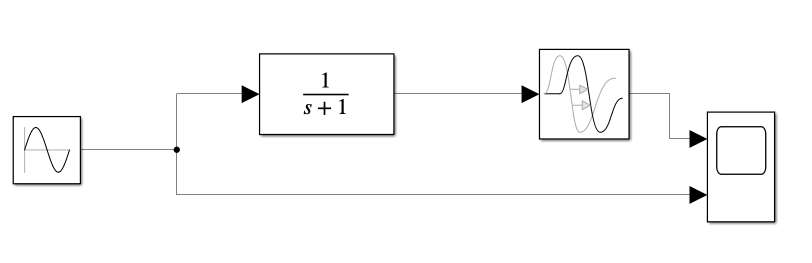
\includegraphics[width=0.8\textwidth]{Bilder/SimulinkEinfach.png}
    \caption{Darstellung des Systems anhand der Übergangsfunktion}
 \end{figure}
Die andere Möglichkeit ist, das System mithilfe von Integratoren darszustellen. Man stellt hierfür die Ein-/Ausgangs-Differentialgleichung nach der höchsten Ableitung um und integriert. Das bietet einem den Vorteil, für die Integratoren Anfangswerte setzen zu können:


 \begin{figure}[H]
    \centering
    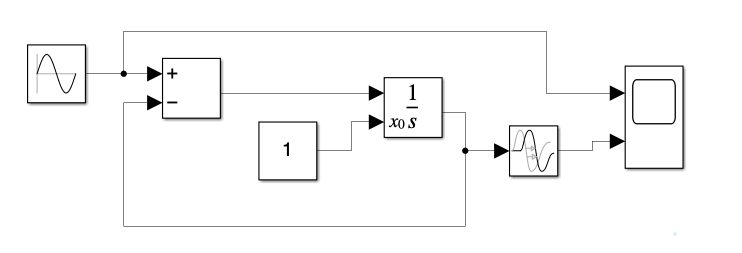
\includegraphics[width=0.8\textwidth]{Bilder/SimulinkKomplex.png}
    \caption{Darstellung des Systems anhand der Ein-/Ausgangs-Differentialgleichung}
 \end{figure}
Die beiden abgebildeten Simulink-Schlatungen führen bei gleicher Eingangsfunktion auf die gleiche Ausgangfunktion.
Mit einem Klick auf den Oszillator wird diese Ausgangsfunktion sowie die am Eingang anliegende Sinus-Funktion in Form eines Graphen ausgegeben (siehe Abbildung 9 \& 10). Dabei ist die blaue Linie die Sinus-Funktion am Eingang mit einer entsprechenden Frequenz $\omega$ in $\frac{rad}{s}$ und die rote Linie die Antwort $y(t)$ unseres Systems.

 \begin{figure}[H]
    \centering
    \begin{minipage}{.5\textwidth}
      \centering
      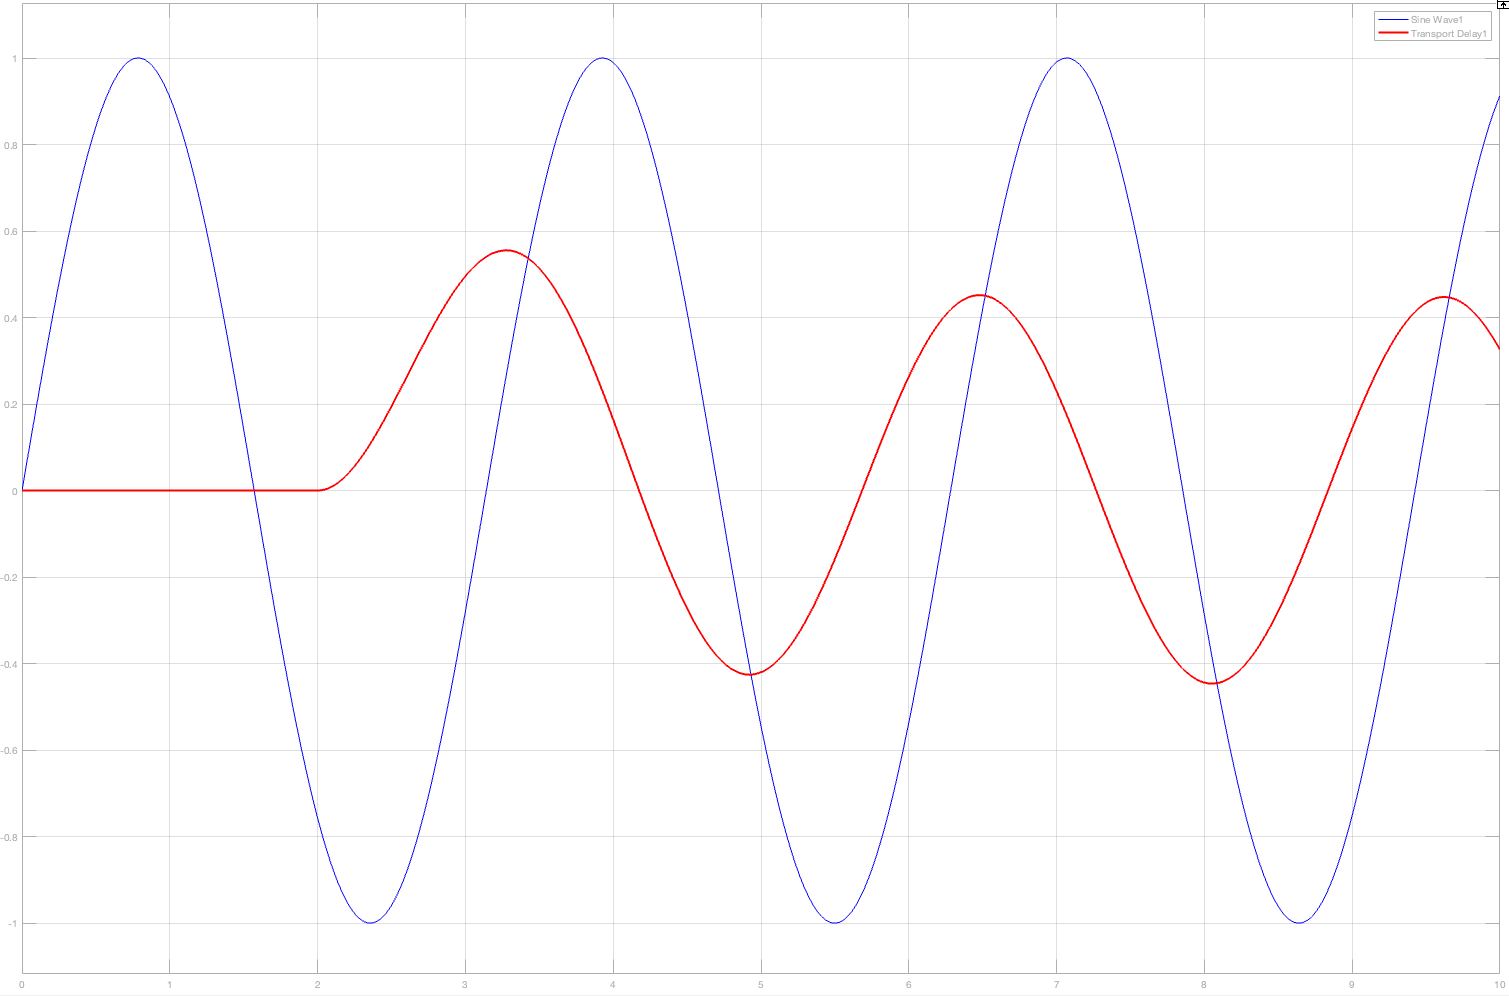
\includegraphics[width=0.9\linewidth]{Bilder/SimulinkOmega2.png}
      \captionof{figure}{Systemantwort bei $\omega = 2$}
    \end{minipage}%
    \begin{minipage}{.5\textwidth}
      \centering
      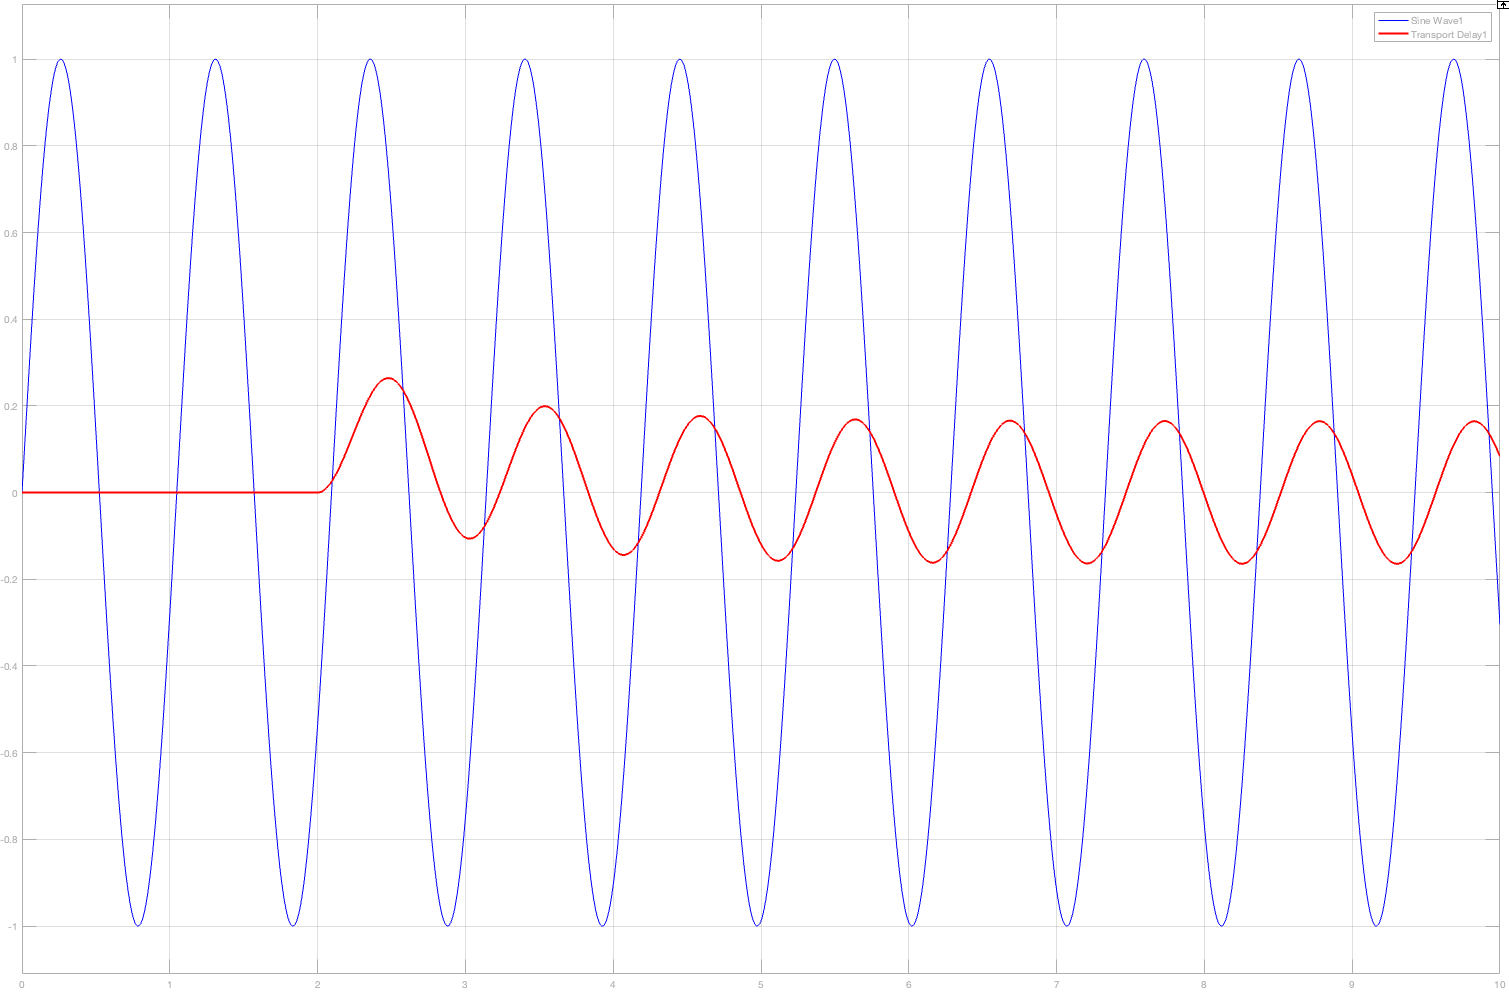
\includegraphics[width=0.9\linewidth]{Bilder/SimulinkOmega6.png}
      \captionof{figure}{Systemantwort bei $\omega = 6$}
    \end{minipage}
\end{figure}

\subsection{Vergleich Bode-Plot, Simulink und Handrechnung}
Im Folgenden werden die Phasenverschiebung und Amplitudenverstärkung unseres Systems anhand des Bode-Diagramms, der Simulink-Schaltung und einer Handrechnung betrachet und anschließend verglichen. Exemplarisch dient dabei die Frequenz $\omega_0 = 6 \frac{rad}{s}$.

Erhält das System ein Eingangssignal $u(t) = A \cdot sin(\omega f + \phi)$, so gilt für den Ausgang:
\begin{align*} 
    y(t) &= Eigenvorgang + y_{stat}(t)
\end{align*}
Wobei für die Statik-Information $y_{stat}$ gilt:
\begin{align*}
    y_{stat}(t) &= |\mathcal{G}(j\omega_0)| \cdot A \cdot sin(\omega_0 t+\phi_0 + arg \enspace \mathcal{G}(j\omega_0))
\end{align*}

Dabei entspricht $|\mathcal{G}(j\omega_0)|$ der Amplitudenverstärkung und $arg \enspace \mathcal{G}(j\omega_0)$ der Phasenverschiebung.

\subsubsection{Handrechnung}
Berechnung des Frequenzgangs:
\begin{align*} 
    \mathcal{G}(s) &=  \frac{1}{s+1}\cdot e^{-2s} \\
    \mathcal{G}(j\omega) &=  \frac{1}{j\omega+1} \cdot e^{-2j\omega} \\
\end{align*} 
Berechnung der Amplitudenverstärkung für $ \omega_0 = 6$: 

Für den Betrag eines Bruchs gilt: $BetragBruch = BetragZ\ddot ahler / BetragNenner$ \\
Für den Betrag von $e^{-aj}$ gilt: $e^{-aj} = 1$
\begin{align*} 
    \mathcal{G}(j6) &=  \frac{1}{6j+1} \cdot e^{-2j\cdot 6}\\
    |\mathcal{G}(j6)| &=  \Bigl| \frac{1}{6j+1} \cdot e^{-12j}\Bigr| \\
    |\mathcal{G}(j6)| &=  \frac{1}{\sqrt{37}}\cdot 1 \approx 0.1644 \\
\end{align*} 
Berechnung der Phasenverschiebung für $ \omega_0 = 6$: 

Für das Argument $arg$ eines komplexen Bruches gilt: 

\quad \quad $arg(\frac{a + bj}{c + dj}) = WinkelZ\ddot ahler - WinkelNenner = arctan\frac{b}{a} - arctan\frac{d}{c}$

Für das Argument $arg$ einer Zeitverzögerung gilt: $arg \enspace e^{-aj} = -a$
\begin{align*} 
    arg \enspace \mathcal{G}(j6) &=   arctan \Bigl( \frac{0}{1} \Bigl) - arctan \Bigl( \frac{6}{1} \Bigl) -12  \\
    arg \enspace \mathcal{G}(j6) &\approx  0-1.4-12 = -13.4 \\
             \Rightarrow  -13.4 \cdot \frac{180}{\pi} & \approx -768.726^{\circ}
\end{align*} 

\subsubsection{Bode-Plot}
\begin{figure}[H]
    \label{fig:bodePlot}
    \label{fig:lassmich}
    \centering
    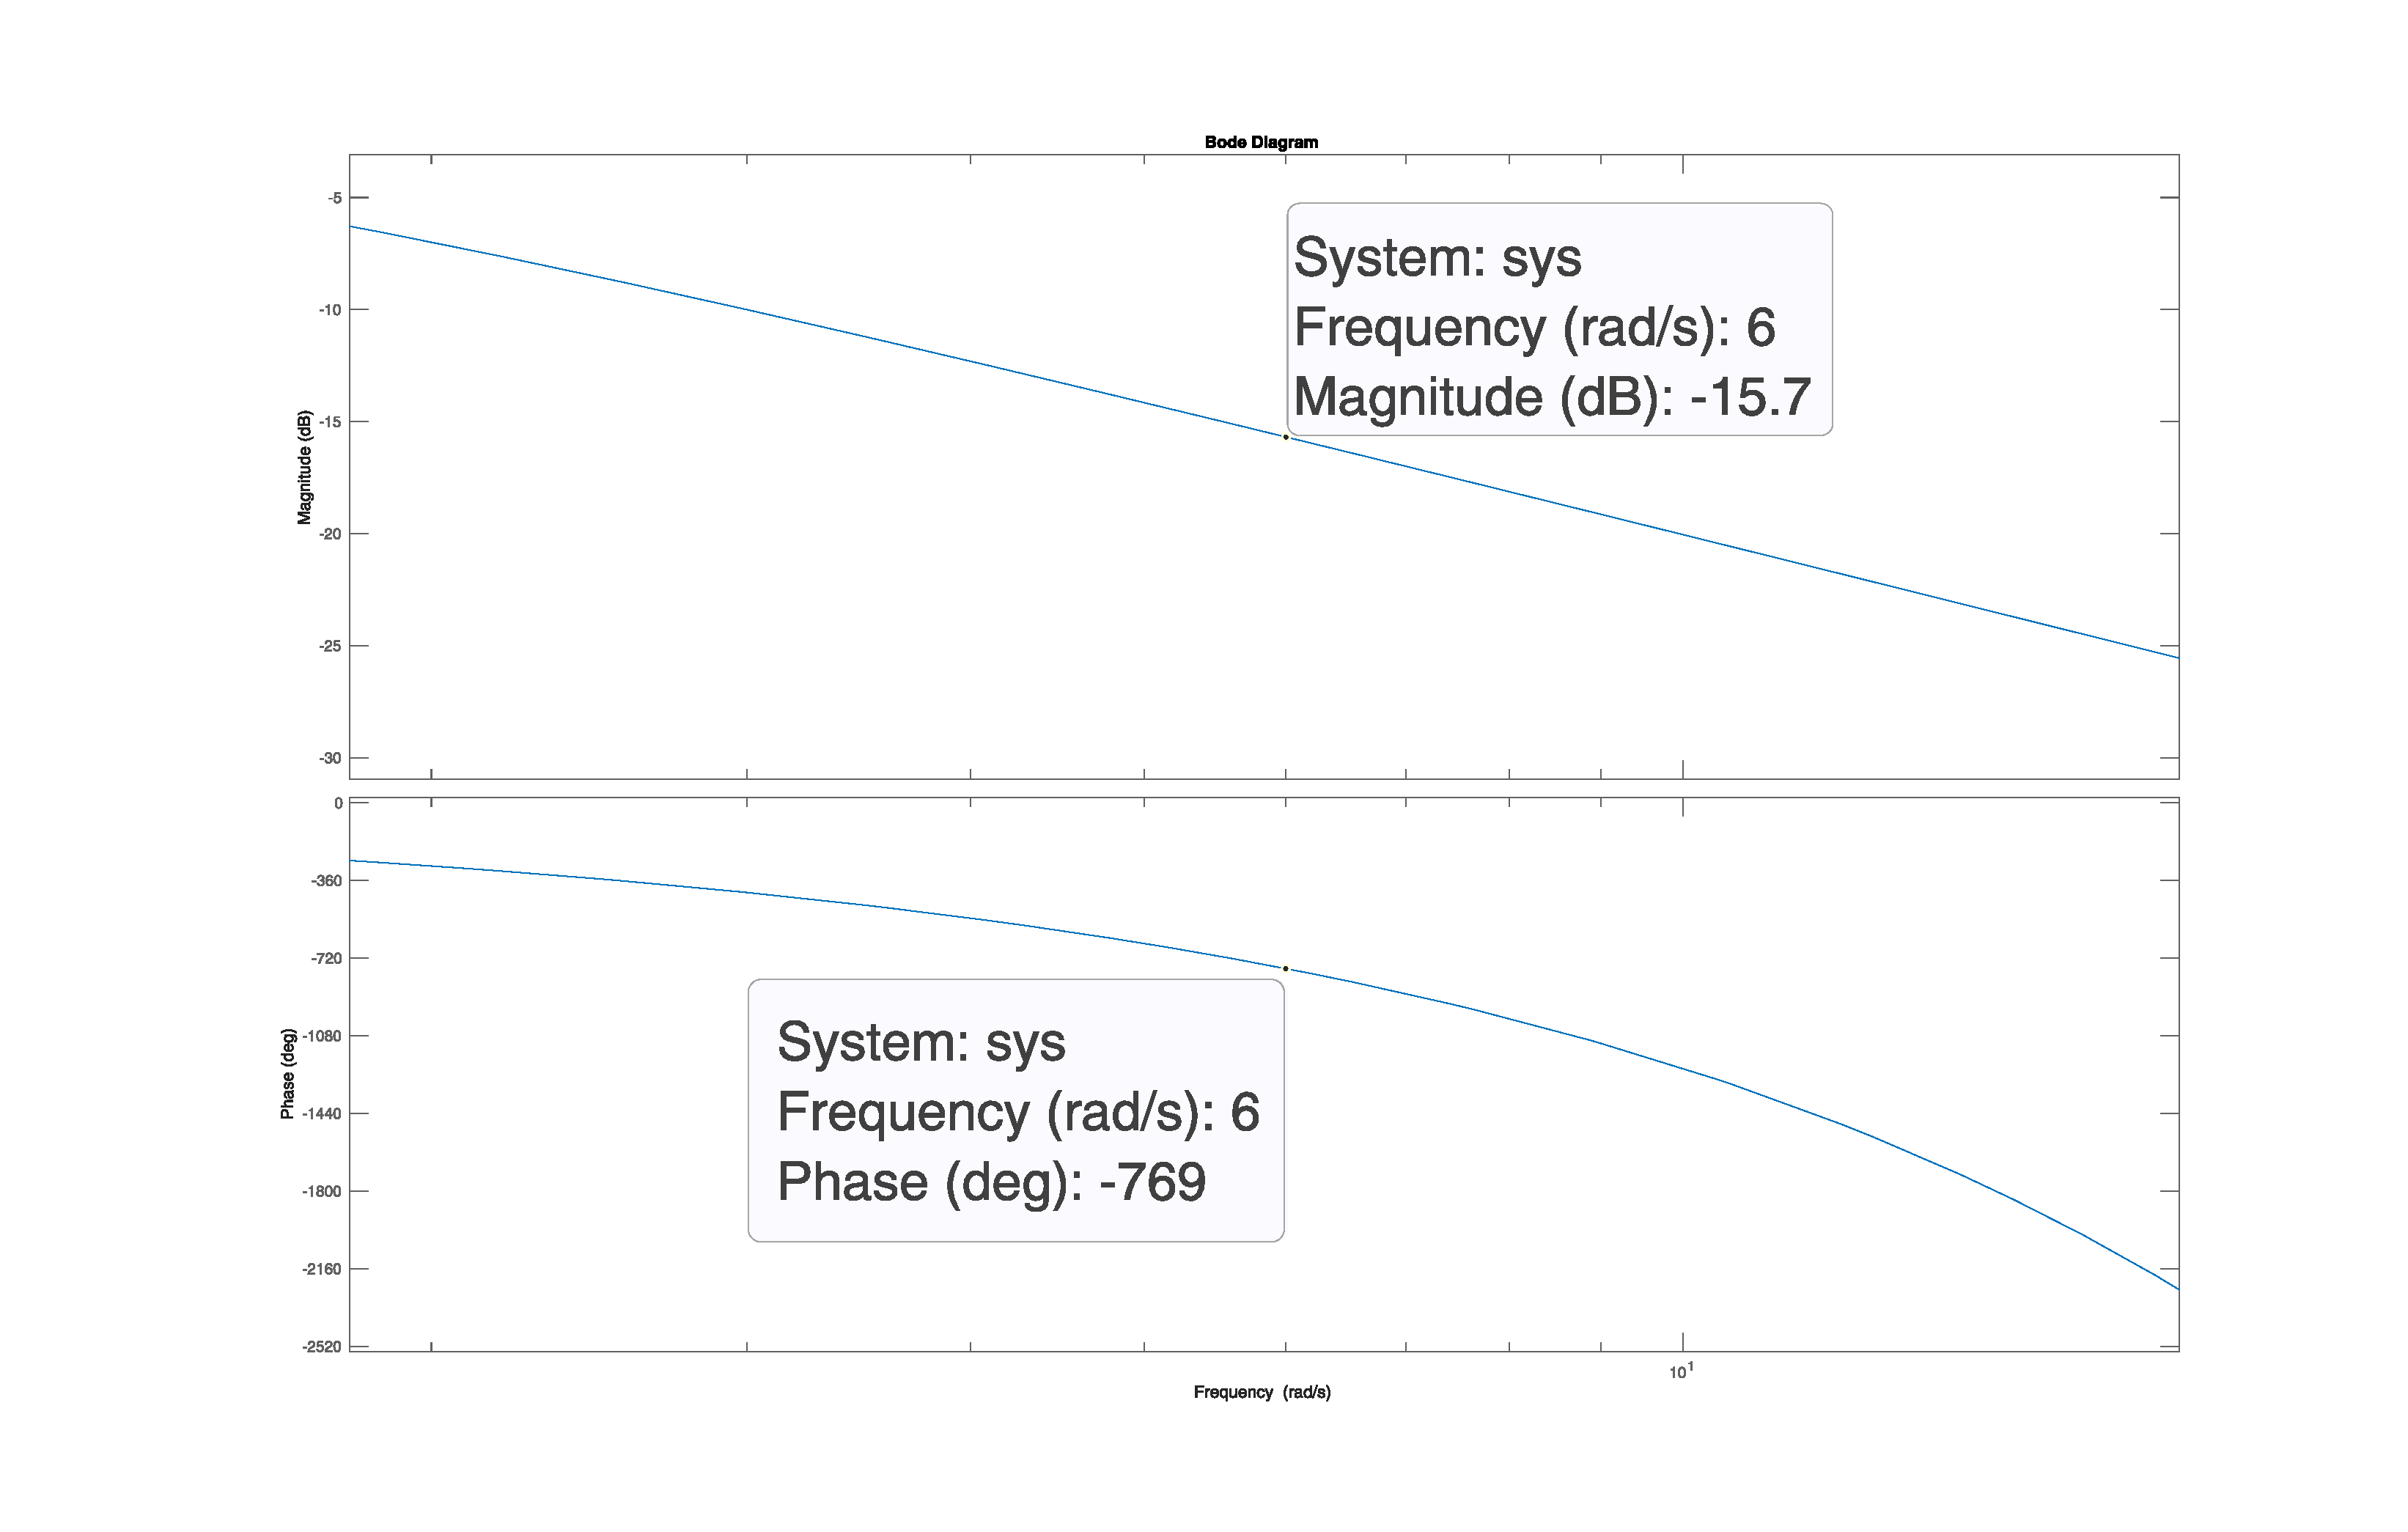
\includegraphics[width=0.8\textwidth]{Bilder/bodeMitZeichen.eps}
    \caption{Bode-Plot mit Zusatzinformationen an der Stelle $ \omega_0 = 6$}
 \end{figure}

Im Bodeplot lässt sich im oberen Bild für $\omega_0 = 6$ eine Verstärkung von $-15.7 dB$ ablesen. Daraus lässt sich der Verstärkungsfaktor errechnen:
\begin{align*}
    20 log(\mathcal{K}) &= - 15.7\\
        \mathcal{K} &= 10^{-\frac{15.7}{20}}\\
        \mathcal{K} & \approx 0.1640
\end{align*}

Im unteren Bild lässt sich für die Phasenverschiebung ein Winkel von $-769^{\circ}$ ablesen.


\subsubsection{Simulink}

%Der aus der Übertragungsfunktion errechnete Wert von $0.1644$ entspricht mit einer minimalen Abweichung dem Wert, der sich aus dem Bode-Diagramm ablesen lässt. 
%Dieder Wert lässt sich ebenfalls graphisch aus dem Simulink-Plot ablesen:

\begin{figure}[H]
    \centering
    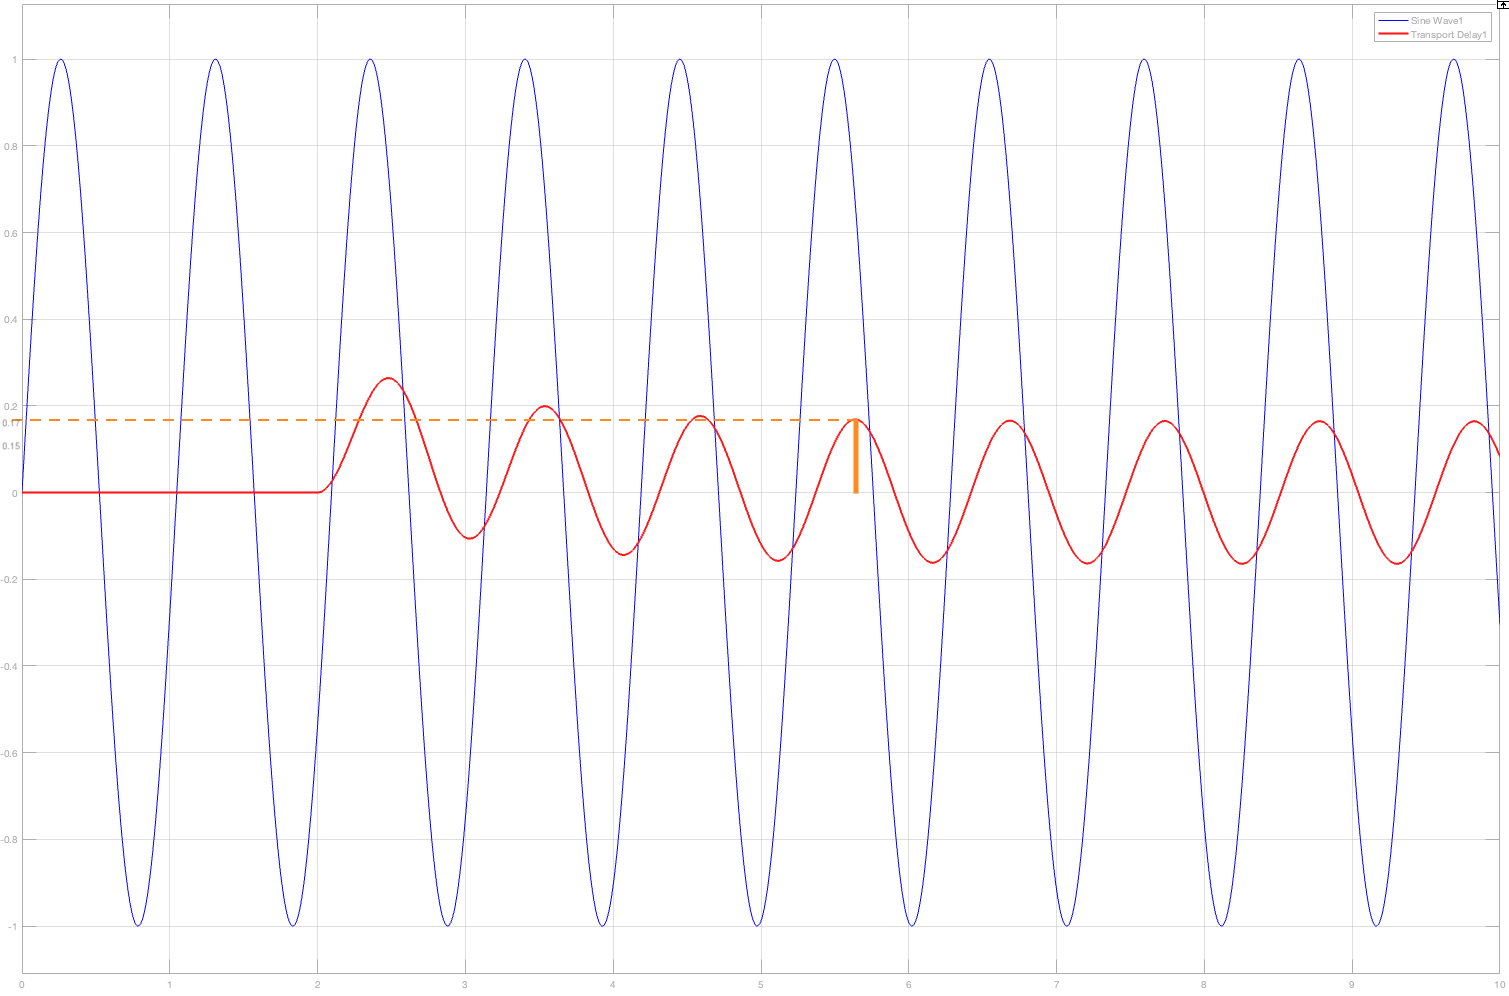
\includegraphics[width=0.6\textwidth]{Bilder/Simulink-Amplitude.png}
    \caption[width=0.6\textwidth]{Messung der Amplitudenverstärkung der eingeschwungnen Ausgansfunktion}
 \end{figure}
 Aus dem Simulink-Ergebnis lässt sich ablesen, dass die Amplitudenverstärkung bei eingeschwungener Ausgangsfunktion ungefähr 0.17 beträgt.

 \begin{figure}[H]
    \centering
    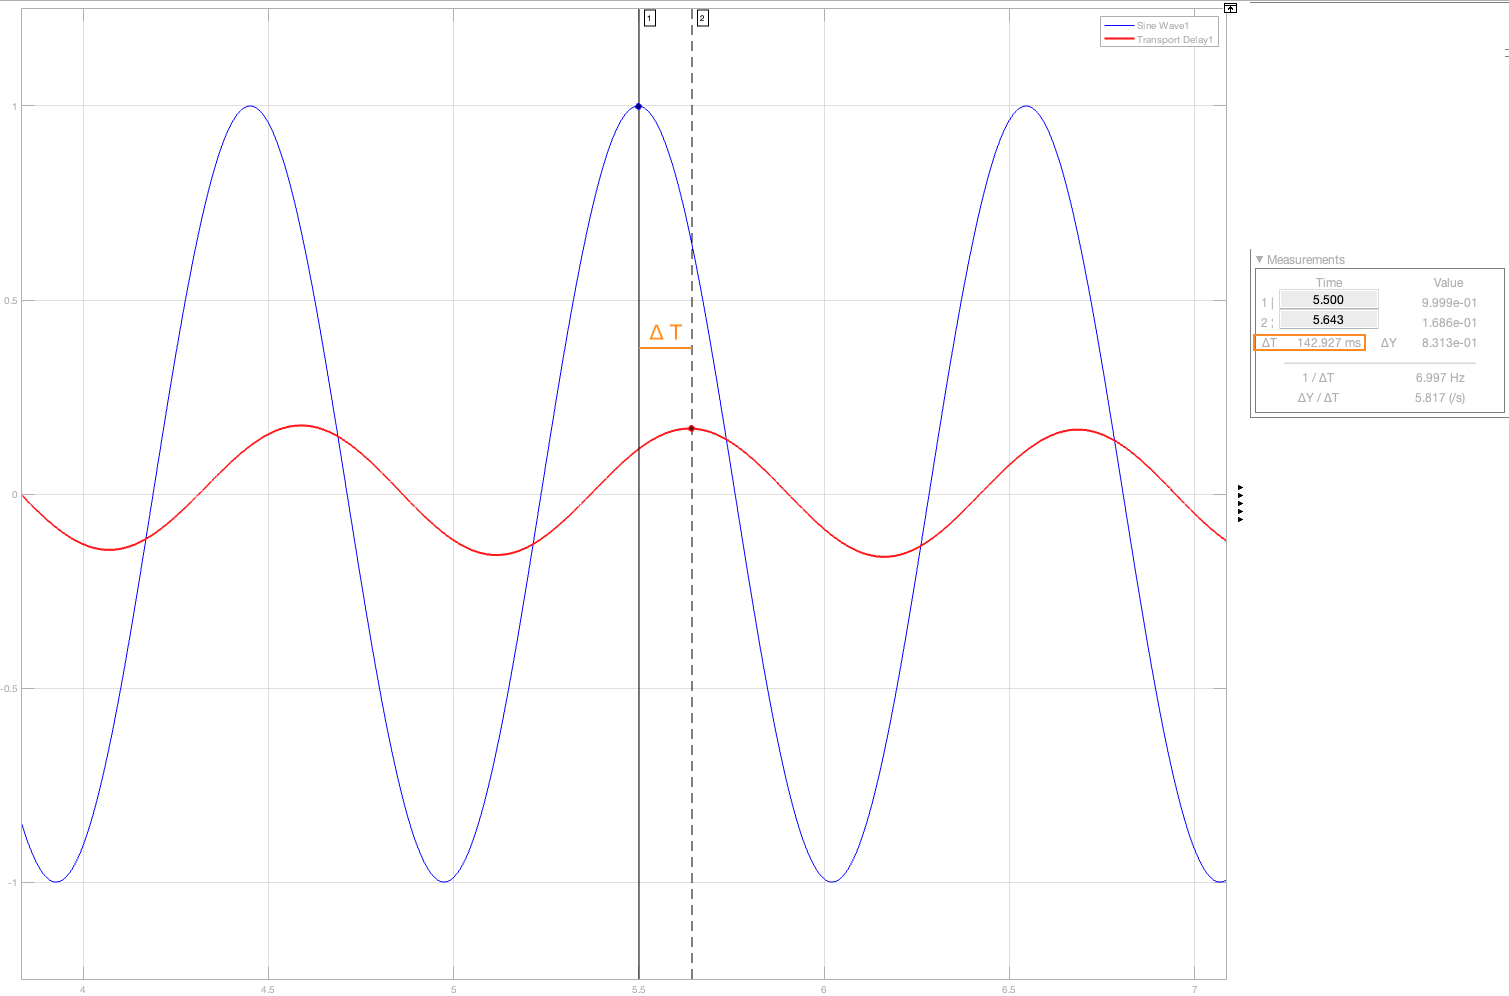
\includegraphics[width=0.6\textwidth]{Bilder/SimulinkPhase.png}
    \caption[width=0.6\textwidth]{Messung der Zeitdifferenz zwischen der \\ Sinusschwingung und der eingeschwungenen Ausgangsfunktion}
 \end{figure}

Die Phasenverschiebung in Grad wird berechnet durch $\phi = (\frac{\Delta t}{T} +T_t ) \cdot 360^{\circ}$, wobei $T$ die Periodendauer ist, die mithilfe von $T = \frac{2\pi}{\omega} = \frac{2\pi}{6} = \frac{\pi}{3}$ ausgerechnet werden kann.

Aus dem Simulink-Plot kann ein $\Delta t = 0.142s$ abgelesen werden.\\
Alle Werte werden in die Formel eingsetzt:
\begin{align*}
    \phi &= (\frac{\Delta t}{T} +T_t ) \cdot 360^{\circ} \\
    \phi &= (\frac{0.142 \cdot 3}{\pi} +2 ) \cdot 360^{\circ} \\
    \phi & \approx 768.81^{\circ}
\end{align*}
%Folglich stimmt die abgelesene Phasenverschiebung aus Simulink mit der per Hand errechneten Lösung, sowie der Lösung aus dem Bode-Diagramm überein.
\subsubsection{Vergleich}
In der folgenden Tabelle sind die einzelnen Werte aus den verschiedenen Ermittlungen miteinander verglichen:
\renewcommand{\arraystretch}{1.2}
\begin{center}
    \begin{tabular}{ c|c|l } 
    Ermittlung & Amplitudenverstärkung & Phasenverschiebung \\
    \hline
    Handrechnung & $0.1644$ & $768.726^{\circ}$ \\ 
    Bode-Plot & 0.1640 & $769^{\circ}$ \\ 
    Simulink & 0.17 & $768.81^{\circ}$ \\ 
    \end{tabular}
\end{center}
Es ist zu erkennen, dass die Werte mit minimalen Abweichungen (Rundungsfehler) übereinstimmen. Das bedeutet, dass unsere Rechnungen und Simulationen richtig sind. 



%SImulationsscheme
%Für 2 Frequenzen ausführen, Amplitudenverstärkung und Phasenverstärkung ablesen
%ERgebnis vergleichen mit Bode-Diagramm
%Ergebnis vergleichen mit Handrechnungen  -> Muss das gleiche herauskommen

%Danach gleiche Schaltung in Integratorform
%Bei diesem Bild kann man anderes Eingangssignal wählen und bei Integratoren die Anfangswerte %angegebenFormel hinschreiben

\subsection{Statische Kennlinie}
Der Verlauf der statischen Kennlinie ist abhängig vom Übertragungsverhalten des Systems. Für P-Verhalten ist die statische Kennlinie eine Ursprungsgerade mit der Steigung $K$, für P-Verhalten eine Gerade, die der x-Achse entspricht, und für I-Verhalten lässt sich formal keine statische Kennlinie angeben.

Da es sich bei unserem System um ein System mit proportionalen Übertragungsverhalten handelt, entspricht die statische Verstärkung $\mathcal{K} = G(0)$ bzw. $\mathcal{K} = \lim_{t\to \infty} h(t)$. Diese lässt sich in Matlab auch mit dem Befehl \texttt{dcgain(sys)} berechnen. \\
Somit ergibt sich bei unserem System eine Ursprungsgerade der Steigung 1 als statische Kennlinie. 

In weniger trivialen Fällen lässt sich die statische Kennlinie folgendermaßen aufnehmen: Man stellt einen konstanten Wert $c$ für $u(t)$ ein, wartet bis alle Eigenvorgänge abgeklungen sind und liest dann den zugehörigen y-Wert ab. Dies wiederholt man für verschiedene $c$ und verbindet schließlich alle Punkte durch eine Line, welche letztendlich die statische Kennlinie darstellt. Dieses Verfahren erklärt, wieso bei instabilen System keine statische Kennlinie gezeichnet werden kann: Diese schwingen sich nie ein, die Eigenvorgänge klingen nie ab.

Noch ein anderer Weg, die statische Verstärkungsmatrix $K$ auszurechnen (im mehrvariablen Fall ist $K$ eine Matrix, die die jeweiligen statischen Verstärkung der einzelnen Eingangssignale angibt), verwendet die Zustandsmatrizen. \\
Dabei wird die Ableitung von $x$ gleich 0 gesetzt, die Gleichung umgestellt, und in die Gleichung von $y$ eingesetzt. Stellt man diese Gleichung erneut um, erhält man K:
\begin{align*}
\dot x &= Ax + Bu \\
0 &\stackrel{!}{=} Ax + Bu \\
x &= -A^{-1}Bu\\ \\
y &= Cx + Du \\
y &= C(-A^{-1}Bu) + Du \\
y &:= Ku \\
K &= -CA^{-1}B + D
\end{align*}

Mithilfe des Matlab-Befehls \texttt{fplot(@(x) 1 * x)} lässt sich unsere statische Kennlinie graphisch darstellen. 

\begin{figure}[H]
    \label{fig:staticCurve}
    \centering
    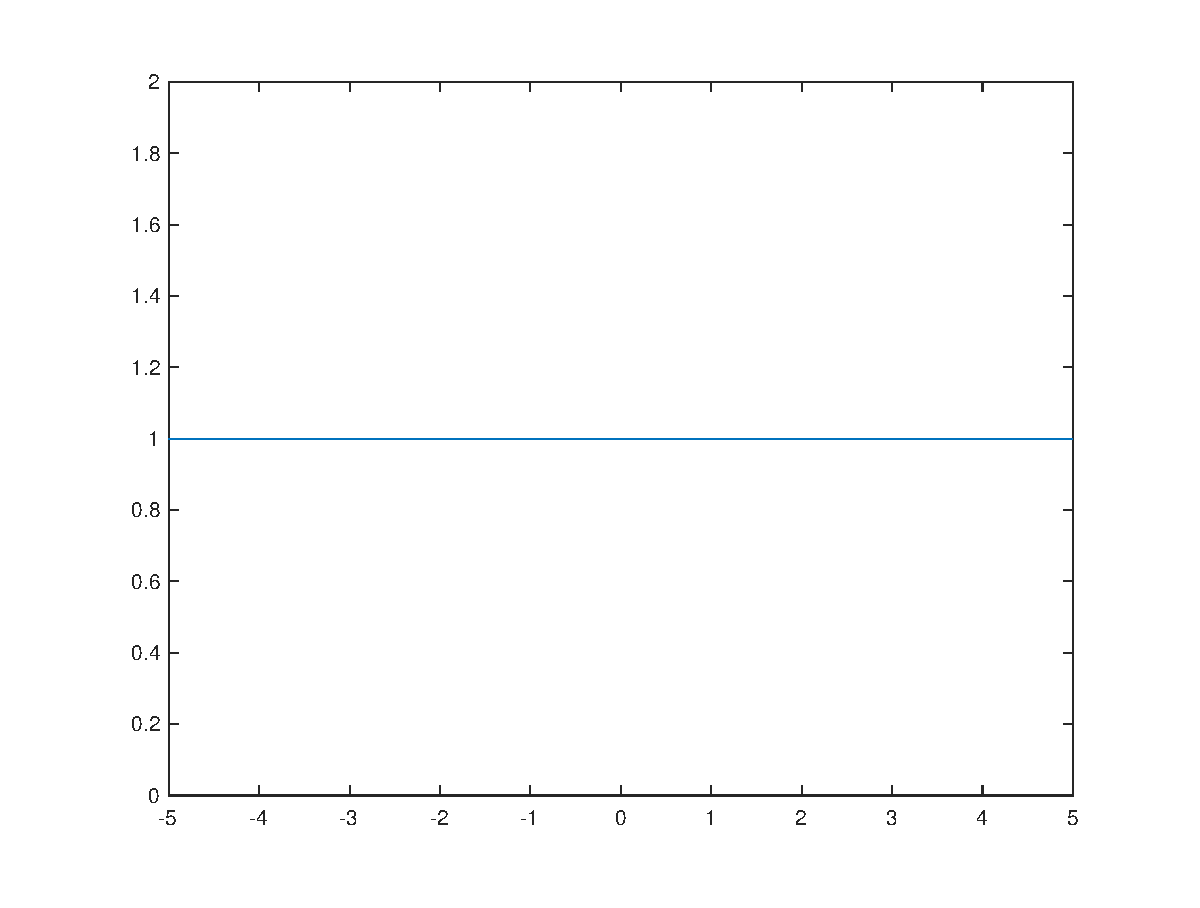
\includegraphics[width=0.8\textwidth]{Bilder/StaticCurvePT1Tt.eps}
    \caption{Statische Kennlinie}
 \end{figure}

Bei Systemen mit einem Eingang und zwei Ausgängen verwendet man stattdessen ein 2-Balken-Diagramm, bei zwei Eingängen und einem Ausgang wird eine Eingangsgröße diskret und die andere kontinuierlich dargestellt, wodurch sich eine Funktionenschar ergibt. 

Der Nachteil der statischen Kennlinie ist, dass sie im Gegensatz zum Pol-Nullstellen-Plot keine Dynamik-Informationen enthält.

\subsection{Pol-Nulstellen-Plot}
Abbildung 15 zeigt den Pol-Nulstellen-Plot zu unserem System. Der passende Matlab-Befehl hierfür lautet \texttt{pzplot(sys)}. Matlab markiert mit \textbf{o} die Nullstellen und mit \textbf{x} die Polstellen des Systems (doppelte Polstellen mit doppel-\textbf{x}).

In unserem Fall hat das System aber keine Nulstellen, da der Zählergrad 0 ist, weshalb in der Abbildung kein \textbf{o} zu sehen ist. Da der Nenner unseres Systems aber den Grad 1 mit $1 + s$ ist, hat unserer System eine reale Polstelle bei $s = -1$, was in der Abbildung mit den \textbf{x} gekennzeichnet ist. 

Aufgrund dieses negativen Realteils handelt es sich um eine grenzstabile Polstelle. Würden alle Polstellen in der offenen linken Halbebene liegen, wäre das System stabil. Da die Polstelle genau auf der Imaginärachse liegt, nennt man das System grenzstabil.

\begin{figure}[H]
    \centering
    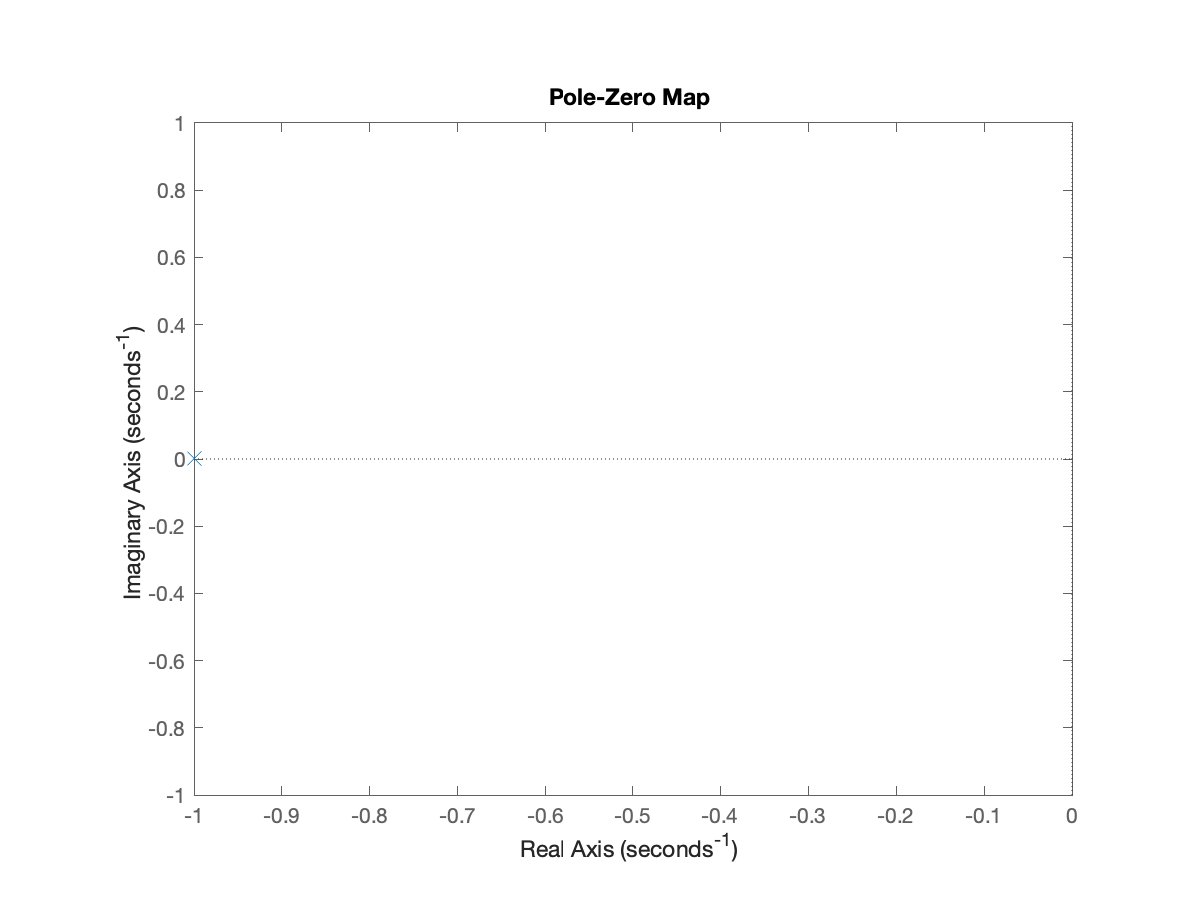
\includegraphics[width=0.8\textwidth]{Bilder/PoleZeroPT1Tt.eps}
    \caption{Pol-Nulstellen-Plot}
 \end{figure}

 Die Pole der Übertragungsfunktion korrespondieren mit den Eigenwerten der System-Matrix $A$ unter der Voraussetzung, dass das System vollständig steuerbar und beobachtbar ist.
 Das heißt, dass keine Pol-Nullstellen-Kürzung auftreten darf.
 In unserem System ist das unkompliziert: Unsere System-Matrix $A$ enthält nur das Element $-1$ und passt somit zur Polstelle $s = -1$.

 Der Nachteil des Pol-Nullstellen-Plots ist, dass er im Gegensatz zur statischen Kennlinie keine Information über die statische Verstärkung enthält.

 %Warum auch immer muss hier das Label nach die Figure und nicht da rein, sonst haben wir ein Problem

